%\documentclass{book}\usepackage{sjtfonts}\usepackage{includegraphics}\usepackage{alltt}\usepackage{latexsym}
%\usepackage{array}
%\begin{document}\input{defs0}%		miradefs.tex 		    June 1994

% opening and closing a quoted Miranda section

\newcommand{\mira}{\noindent\hrulefill\nopagebreak\so}
\newcommand{\arim}{\nopagebreak\st\hrulefill\\}

% backslash in the Miranda environment
% Only feasible approach is to use \verb+\+
% in line!

%\newcommand{\bs}{$\mi\backslash\!\!$}
%\newcommand{\lbs}{\mbox{\verb+\+}}

% ignoring part of the input

\newcommand{\ignore}[1]{}

% a blank line in a Miranda section

\newcommand{\bl}{\mbox{\ }}

% Signalling a diffculty.

\definecolor{light-gray}{gray}{0.95}

\newcommand{\beware}[2]
 {\medskip\noindent\colorbox{light-gray}{\parbox{\textwidth}
 {\mbox{\large\textbf{#1}} \medskip\noindent\\ #2}\medskip\noindent}}

% Subscripting in Miranda text
\newcommand{\subscr}[2]{\mbox{${\mbox{\texttt{#1}}}_{\mbox{\texttt{#2}}}$}}

%\newcommand{\subscr}[2]{\mbox{${\mbox{\mi #1}}_{\mbox{\smtt #2}}$}}
\newcommand{\aone}{\subscr{a}{1}}
\newcommand{\atwo}{\subscr{a}{2}}
\newcommand{\ak}{\subscr{a}{k}}

\newcommand{\aoneone}{\subscr{a}{1,1}}

\newcommand{\eone}{\subscr{e}{1}}
\newcommand{\etwo}{\subscr{e}{2}}
\newcommand{\ei}{\subscr{e}{i}}
\newcommand{\er}{\subscr{e}{r}}

\newcommand{\fone}{\subscr{f}{1}}
\newcommand{\fl}{\subscr{f}{l}}

\newcommand{\gone}{\subscr{g}{1}}
\newcommand{\gtwo}{\subscr{g}{2}}
\newcommand{\gi}{\subscr{g}{i}}
\newcommand{\gr}{\subscr{g}{r}}

\newcommand{\hone}{\subscr{h}{1}}
\newcommand{\hl}{\subscr{h}{l}}

\newcommand{\pone}{\subscr{p}{1}}
\newcommand{\ptwo}{\subscr{p}{2}}
\newcommand{\pk}{\subscr{p}{k}}

\newcommand{\qone}{\subscr{q}{1}}
\newcommand{\qtwo}{\subscr{q}{2}}
\newcommand{\qk}{\subscr{q}{k}}

\newcommand{\rone}{\subscr{r}{1}}
\newcommand{\rtwo}{\subscr{r}{2}}

\newcommand{\tone}{\subscr{t}{1}}
\newcommand{\ttwo}{\subscr{t}{2}}
\newcommand{\tn}{\subscr{t}{n}}

\newcommand{\vone}{\subscr{v}{1}}
\newcommand{\vtwo}{\subscr{v}{2}}
\newcommand{\vn}{\subscr{v}{n}}

% for regular expressions

\newcommand{\stone}{\subscr{st}{1}}
\newcommand{\sttwo}{\subscr{st}{2}}
\newcommand{\stn}{\subscr{st}{n}}
\newcommand{\rthree}{\subscr{r}{3}}

\newcommand{\eps}{$\varepsilon$}
\newcommand{\trans}[1]{\stackrel{\mbox{\tt #1}}{\longrightarrow}}



% superscript in Miranda text

\newcommand{\superscr}[2]{\mbox{${\mbox{\mi #1}}^{\mbox{\smtt #2}}$}}

% Not equals in Miranda text

\newcommand{\noteq}{\makebox[0pt][l]{=}/}
\newcommand{\overslash}{\makebox[0pt][l]{/}}

% Definitions in complexity chapter

\newfont{\oldSym}{cmsy10}
\newcommand{\Th}{\boldmath$\oldSym\Theta$}
\newcommand{\pow}[1]{\^{}#1}
\newcommand{\leqq}{$\leq$}
\newcommand{\geqq}{$\geq$}
\newcommand{\lll}{$\ll$}
\newcommand{\eqq}{$\equiv$}
\newcommand{\ltwo}{\subscr{log}{2}}

% Indexing

\newcommand{\minx}[1]{\index{#1@{\ttfamily{}#1}}}
\setcounter{chapter}{10}\setcounter{page}{191}






\chapter{Developing higher-order programs}
\chapstart
\label{moreDesign}
\label{developingHOPs}
\index{program development|(}
\index{higher-order function!defining HOFs|(}



This chapter doesn't introduce any new Haskell features; instead it gives a series of examples, exercises and case studies which build on what we have covered so far. In particular it uses what we have learned about higher-order functions in the previous chapter.

As we saw there, functions in Haskell are data values just like any other, and so they can be used in modelling just as easily as using other data types. This is completely different from other kinds of programming languages, such as Java, C or C\#, where there is a rigid distinction between data and the methods operating over that data. We'll see that having functions as data gives us a powerful new tool for programming, and that is illustrated in this chapter through a series of examples and exercises.

We also include in this chapter a longer example  -- building an index for a document -- which shows how program development can proceed in Haskell, using higher-order functions as a natural part of the development of larger programs. We start the chapter by revisiting the \texttt{Picture} example, and conclude with some general advice about program development, and about how to read and understand an unfamiliar function definition in Haskell. 




\section{Revisiting the \texttt{Picture} example}
\markright{Revisiting the \texttt{\runinghead Picture} example}
\label{hofPicture}
\index{pictures|(}

Now that we have been introduced to higher-order functions, and in particular partial 
application, we can revisit the example of pictures  and complete our
definitions of the functions over the \texttt{Picture} type. The case
study was introduced in
Chapter \ref{intro} and further
developed in Sections \ref{picModuleEx} and \ref{picturesAgain}.

Recall that a picture is a list of lines, each of which is made up of a
list of characters
\begin{alltt}
type Picture = [[Char]]
\end{alltt}
We first define reflection in a horizontal mirror, which is given simply
by reversing the list of lines,
\begin{alltt}\minx{flipH}
flipH :: Picture -> Picture
flipH = reverse
\end{alltt}
To reflect in a vertical mirror we need to reverse every line -- clearly
a task for \texttt{map}:
\begin{alltt}\minx{flipV}
flipV :: Picture -> Picture
flipV = map reverse
\end{alltt}
To place pictures next to each other we have two functions. To put one
picture above
the other we join together the two lists of lines
\begin{alltt}\minx{above}
above :: Picture -> Picture -> Picture
above = (++)
\end{alltt}
while placing the pictures side-by-side requires corresponding lines to
be joined together with \texttt{++}, using the function \texttt{zipWith}
first introduced in Section \ref{hofs}.
\begin{alltt}\minx{beside}
beside :: Picture -> Picture -> Picture
beside = zipWith (++)
\end{alltt}
Among the other functions mentioned were 
\begin{alltt}
invertColour :: Picture -> Picture
superimpose  :: Picture -> Picture -> Picture
printPicture :: Picture -> IO ()
\end{alltt}
and we give their definitions now. To invert the colour in a picture, we
need to invert the colour in every line, so
\begin{alltt}\minx{invertColour}
invertColour = map ...
\end{alltt}
where \texttt{...} will be the function to invert the colour in a
single line.
To invert every character in a line -- which is itself a list of
characters -- we will again use \texttt{map}. The function mapped is
\texttt{invertChar}, first defined in Section \ref{picturesAgain}. This gives
the definition 
\begin{alltt}\minx{invertChar}
invertColour :: Picture -> Picture
invertColour = map (map invertChar)
\end{alltt}
which we can read as saying
\begin{quote}
apply \texttt{map invertChar} to every line in the \texttt{Picture};
that is, apply the function \texttt{invertChar} to every character in the
\texttt{Picture}, which is a list of lists of characters.
\end{quote}
Suppose we are equipped with a function
\begin{alltt}\minx{combineChar}
combineChar :: Char -> Char -> Char
\end{alltt}
which superimposes two characters; how are we to use this in
superimposing two pictures? Recall the function 
\begin{alltt}
zipWith :: (a -> b -> c) -> [a] -> [b] -> [c]
\end{alltt}
where \texttt{zipWith f xs ys} produces a list by applying the function \texttt{f}
to corresponding elements chosen from \texttt{xs} and \texttt{ys}, so that, for instance
\begin{alltt}
zipWith (*) [2,0] [3,1] = [6,0]
\end{alltt}
To superimpose the pictures, we will need to
superimpose corresponding lines, so
\begin{alltt}\minx{superimpose}
superimpose = zipWith ...
\end{alltt}
where \texttt{...} will be required to superimpose two single lines. 

In doing this, we have to superimpose corresponding
characters, so this is again an application of \texttt{zipWith}. What is
used to perform the combination of individual characters? The answer is 
\texttt{combineChar}, and so we have
\begin{alltt}
superimpose :: Picture -> Picture -> Picture
superimpose = zipWith (zipWith combineChar)
\end{alltt}

Our final definition is of \texttt{printPicture}, which outputs a \texttt{Picture}
to the screen. We have already seen that to output a \texttt{String}
we can use the function
\begin{alltt}
putStr :: String -> IO ()
\end{alltt}
so it will be sufficient for us to precede application of this by a function
to turn the list of lines making up the \texttt{Picture} into a string,
in which the lines are separated by newline characters. This we can write
as a composition
\begin{alltt}
concat . map (++"\bs{n}")
\end{alltt}
since the effect of this is first to add a newline character to every
line -- the role of \texttt{map (++"\bs{n}")} -- and then to join this list of 
strings into a single string -- the effect of the \texttt{concat}. We
therefore define the printing function thus:
\begin{alltt}\minx{printPicture}
printPicture :: Picture -> IO ()
printPicture = putStr . concat . map (++"\bs{n}")
\end{alltt}

\begin{exercises}
\item[]\parbox\textwidth{\leftskip -2.8em In these exercises we
suggest further operations over pictures.\par}
\item
Define a function
\begin{alltt}
chessBoard :: Int -> Picture
\end{alltt}
so that \texttt{chessBoard n}
is a picture of an \texttt{n} by \texttt{n} chess board.

\item
How would you implement \texttt{invertColour}, \texttt{superimpose} and
\texttt{printPicture} if \texttt{Picture} was defined to be
\texttt{[[Bool]]}?

\item
Define a function
\begin{alltt}
makePicture :: Int -> Int -> [(Int,Int)] -> Picture
\end{alltt}
where the list argument gives the positions of the black points in the
picture, and the two integer arguments give the width and height of the picture.
For example,
\begin{alltt}
makePicture 7 5 [(1,3),(3,2)]
\end{alltt}
will have the form
\begin{alltt}
.......
...#...
.......
..#....
.......
\end{alltt}
It is evident from this that positions within lines and lines themselves
are counted from zero, with line zero being the top line.

\item
Define a function 
\begin{alltt}
pictureToRep :: Picture -> ( Int , Int , [(Int,Int)] )
\end{alltt}
which has the reverse effect of \texttt{makePicture}. For example, if 
\texttt{pic} is
\begin{alltt}
....
.##.
....
\end{alltt}
then \texttt{pictureToRep pic} will be \texttt{( 4 , 3, [(1,1),(1,2)] )}

\item
If we make the definition
\begin{alltt}
type Rep = ( Int , Int , [(Int,Int)] )
\end{alltt}
discuss how you would define functions over \texttt{Rep} to rotate,
reflect and superimpose 
pictures under this alternative representation. Discuss the advantages
and disadvantages of this representation in comparison with
the original representation given by
the \texttt{Picture} type.

\item
In the light of the discussion in the last four chapters, redo the exercises of 
Section \ref{posPix}, which deal with positioned
pictures.
\index{pictures|)}
\end{exercises}


\section{Functions as data: strategy combinators}
\label{strategyCombs}
\index{function!as data|(}\index{strategies}

This section revisits the Rock - Paper - Scissors game, which we have already looked at in Section \ref{EnumTypes} which introduced the \texttt{Move} type, in Section \ref{strategiesRPS} where we defined the \texttt{Strategy} type, and in Section \ref{playingRPS} where we saw how the game could be played. Strategies are represented by functions
\begin{alltt}\minx{Strategy}
type Strategy = [Move] -> Move
\end{alltt}
Section \ref{strategiesRPS} introduced a number of strategies, including random, cycling and constant strategies. One way of building new strategies is to combine existing strategies in different ways: we do this by defining functions or \textbf{combinators} working over strategies. Because strategies are represented by functions, these new functions will be \emph{higher-order}, having functions as arguments and results.

\index{combinator}
\beware{Why `combinator'?}{
Why do we use the word `combinator'? It's a piece of history that certain functions in the $\lambda$-calculus were called combinators, and this usage has passed over to the functional programming community. Just remember that `combinator' is another word for `function', typically a higher-order function. A `combinator library' is just a library of (higher-order) functions, too.}

\subsection*{Choosing between alternatives}

Let's begin by defining the function
\begin{alltt}\minx{alternate}
alternate :: Strategy -> Strategy -> Strategy
\end{alltt}
so that the strategy given by
\begin{alltt}
alternate str1 str2
\end{alltt}
is to combine the two strategies \texttt{str1} and \texttt{str2}, using them alternately. We can define the function using partial application like this
\begin{alltt}
alternate str1 str2 moves =
    case length moves `rem` 2 of
      1 -> str1 moves
      0 -> str2 moves\end{alltt}
or using a lambda abstraction we have
\begin{alltt}
alternate str1 str2 = 
    \bs{}moves ->
        case length moves `rem` 2 of
          1 -> str1 moves
          0 -> str2 moves
\end{alltt}
In both definitions we check whether the length of list of \texttt{moves} is even or odd to decide between the two alternatives. Another way to define the function is this:
\begin{alltt}
alternate str1 str2 moves = 
    map ($ moves) [str1,str2] !! (length moves `rem` 2) 
\end{alltt}
In this definition both of the strategies -- put into a list -- are applied to the \texttt{moves} and then one of the elements of that list is chosen using \texttt{(length moves `rem` 2)} as an index into the list. In reading this definition, recall that \texttt{xs!!j} is the \texttt{j}th element of \texttt{xs}, starting counting at \texttt{0}, and that \texttt{(\$ moves)} is a partial application of \texttt{\$}, the application operator, so that
\begin{alltt}
($ moves) str1 \step{}(str1 $ moves) \step{}str1 moves
\end{alltt}

\begin{exercises}

\item
Using \texttt{randInt n}, which returns a random integer in the range \texttt{[0 .. n-1]}, or otherwise, define a function
\begin{alltt}
sToss :: Strategy -> Strategy -> Strategy
\end{alltt}
so that \texttt{sToss srt1 srt2} makes a random choice between the two strategies each time the function is applied to a list of moves.

\item
Define a function 
\begin{alltt}
alternativeList :: [Strategy] -> Strategy
\end{alltt}
which cycles through all the strategies in the argument in turn. \emph{Hint:} you may want to model you definition on one of the definitions of \texttt{alternative} above.
You may also want to think about what your function does when passed the empty list of strategies!

\item
Define a function 
\begin{alltt}
sTossList :: [Strategy] -> Strategy
\end{alltt}
which makes a random choice of which strategy it should apply form its argument list, each time it applied. In writing the definition, you will need to think about what \texttt{sTossList []} should be.

\item 
Can you use the function \texttt{sTossList} to give another definition of the \texttt{randomStrategy} strategy first defined in Section \ref{strategiesRPS}?

\end{exercises}

\subsection*{Other strategy combinators}

There are more sophisticated ways of playing Rock - Paper - Scissors than playing randomly or cycling through a set of alternatives. A first approach is to make a hypothesis about what strategy our opponent is playing, and for us to play to beat that. We achieve that by applying our opponent's strategy (here called \texttt{opponent}) and choose to \texttt{beat} that:
\begin{alltt}\minx{beatStrategy}
beatStrategy :: Strategy -> Strategy

beatStrategy opponent moves =
    beat (opponent moves)
\end{alltt} 
We will look at some other suggested strategy combinators in the following exercises.

\begin{exercises}

\item
Define a function
\begin{alltt}
majority :: [Strategy] -> Strategy
\end{alltt}
which works by applying all the strategies in the list at each stage, choosing the option that is chosen by the most strategies: in the case of a draw, a choice is made randomly.

\item
Define a function
\begin{alltt}
train :: Moves -> [Strategy] -> Strategy
\end{alltt}
which is supplied with a list of opponent's moves to train it, and a list of possible strategies to use. The function should run all the strategies in the list on the list of moves, and choose the strategy which is most successful in winning against the given moves. 



\end{exercises}


\section{Functions as data: recognising regular expressions}
\label{regExps}\index{regular expressions|(}

Regular expressions are \emph{patterns} which can be used to describe sets of strings
of characters of various kinds, such as these.
\begin{itemize}
\item The identifiers of a programming language
-- strings of alphanumeric characters
which begin with an alphabetic character.
\item The numbers -- integer or real -- given in a programming language.
\item
Regular expressions can also be used to extend the pattern language in a programming language, allowing functions to match in more powerful ways than those built in.
\end{itemize}
There are five sorts of pattern, or regular expression:

\medskip
\noindent
\begin{tabular}{ll}
\eps & This is the Greek character {\em epsilon}, which matches the
empty string.\\
\tt x & {\tt x} is any character. This matches the character itself.\\
\tt (\rone|\rtwo) & \rone\ and \rtwo\ are regular expressions.\\
\tt (\rone\rtwo) & \rone\ and \rtwo\ are regular expressions.\\
\tt (r)* & {\tt r} is a regular expression.
\end{tabular}

\bigskip
\noindent
Examples of regular expressions include {\tt (a|(ba))},
{\tt ((ba)|(\eps|(a)*))} and {\tt hello}. 
In order to give a more readable 
version of these, it is assumed that {\tt *} binds more tightly than
juxtaposition ({\em i.e.} {\tt (\rone\rtwo)}), and that juxtaposition binds
more tightly than {\tt |}. This means that {\tt \rone\rtwo*} will
mean {\tt (\rone(\rtwo)*)}, {\em not} {\tt ((\rone\rtwo))*}, and that
{\tt \rone|\rtwo\rthree} will mean {\tt \rone|(\rtwo\rthree)}, {\em not} 
{\tt (\rone|\rtwo)\rthree}.

\medskip
\noindent
Regular expressions are patterns, so we need to describe which strings match each
regular expression.

\bigskip
\noindent
\begin{tabular}{lp{4in}}
\eps & The empty string matches epsilon.\\ \ \\
\tt x & The character {\tt x} matches the pattern {\tt x},
for any character {\tt x}. \\ \ \\
\tt (\rone|\rtwo) & The string {\tt st} will match {\tt (\rone|\rtwo)}
if {\tt st}  matches either \rone\ or
\rtwo\ (or both).\\ \ \\
\tt (\rone\rtwo) & The string {\tt st} will match {\tt (\rone\rtwo)}
if {\tt st} can be
split into two substrings \stone\ and \sttwo, {\tt st = \stone++\sttwo}, so
that \stone\ matches \rone\ and \sttwo\ matches \rtwo.\\ \ \\
\tt (r)* & The string {\tt st} will match  {\tt (r)*}
if {\tt st} can be split into 
zero or more substrings, {\tt st = \stone++\sttwo++...++\stn}, each of which
matches {\tt r}. The zero case implies that the empty string will match
{\tt (r)*} for {\em any\/} regular expression {\tt r}.
\end{tabular}

\medskip
\noindent
Let's build a model of regular expressions in Haskell; we choose to embed them as functions from \texttt{String} to \texttt{Bool}, which is the function which recognises exactly the strings matching the pattern.
\begin{alltt}\minx{RegExp}
type RegExp = String -> Bool
\end{alltt}
Now we define the five different kinds of regular expression, starting off with epsilon, $\epsilon$, which is matched by the empty string only. We use an operator section to define the function:
\begin{alltt}\minx{epsilon}
epsilon :: RegExp
epsilon = (=="")
\end{alltt}
We use a similar definition for the function that recognises a single character, passed in as its argument
\begin{alltt}\minx{char}
char :: Char -> RegExp
char ch = (==[ch])
\end{alltt}
We next define the Haskell operator \texttt{|||}, which implements the `or' operation, \texttt{|}. Applying this to \texttt{e1} and \texttt{e2} gives a function which takes the string \texttt{x} to the `or' of the two values \texttt{e1 x} and \texttt{e2 x}: 
\begin{alltt}\minx{"|"|"|}
(|||) :: RegExp -> RegExp -> RegExp

e1 ||| e2 = 
    \bs{}x -> e1 x || e2 x
\end{alltt}
Sequencing the match of two regular expressions is given by the Haskell \texttt{<*>} operator. In defining this we'll use the function \texttt{splits} that returns a list of all the ways that a string can be split in two
\begin{alltt}\minx{splits}
splits "Spy" \step{}[("","Spy"),("S","py"),("Sp","y"),("Spy","")]
\end{alltt}
Now we can give the definition of \texttt{<*>}\minx{<*>}
\begin{alltt}
(<*>) :: RegExp -> RegExp ->  RegExp

e1 <*> e2 =
    \bs{}x -> or [ e1 y && e2 z | (y,z) <- splits x ]
\end{alltt}
How does this definition work? The list comprehension runs through all the splits of the input string, \texttt{x}. For each of these we test whether the front half (\texttt{y}) matches the first pattern (\texttt{e1}) by \emph{applying} \texttt{e1} to \texttt{x}, and similarly we apply \texttt{e2} to the second half of the string (\texttt{z}). Since we need both matches to succeed, we combine the results with `and', \texttt{\&\&}. The result of this is to give a list of the answers for each split: we only need \emph{one} of these to succeed, and so we combine the results with the built-in function \texttt{or} that takes the `or' of a list of Boolean values. 

We can define the star operation using the operators that we've already defined, like this:
\begin{alltt}\minx{star}
star :: RegExp -> RegExp

star p = epsilon ||| (p <*> star p)
\end{alltt}
The definition says 'to match {\tt (p)*}, either match it zero times (\texttt{epsilon}) or match \texttt{p} followed by \texttt{(p)*}'. What is elegant about this is that we just used the operators \texttt{|||} and \texttt{<*>}, together with recursion, to make the definition at the level of the \texttt{RegExp} type; we didn't need to think about \texttt{star p} being a function.

\beware{Getting \texttt{star} right}{
There is a flaw in the definition of \texttt{star} that we have just given: if it is possible for \texttt{p} to match the empty string, i.e. if \texttt{p ""} is \texttt{True}, then the definition may go into an infinite loop. 

\medskip
We need to modify the definition of \texttt{star} to say
instead that   
\begin{alltt}
star p = epsilon ||| (p <**> star p)
\end{alltt}
where \texttt{<**>} is defined like \texttt{<*>} except that it omits the split \texttt{("",st)} from \texttt{splits st}. This change is enough to make sure that the infinite loop is avoided, as it means that the first match of \texttt{p} can't be with an empty string, and so the next match of \texttt{(p)*} must be on a shorter string.}

\begin{exercises}

\item
Define the function
\begin{alltt}
splits :: [a] -> ([a],[a])
\end{alltt}
which defines the list of all the ways that a list can be split in two (see the example of \texttt{splits "Spy"} above).

\item
By trying it with a number of examples, which strings does this regular expression match?
\begin{alltt}
star ((a ||| b) <*> (a ||| b))
\end{alltt}
where \texttt{a} and \texttt{b} are defined by
\begin{alltt}
a, b :: RegExp
a = char 'a'
b = char 'b'
\end{alltt}

\item
Which strings does this regular expression match?
\begin{alltt}
star (star ((a ||| b) <*> (a ||| b)))
\end{alltt}
 
\item
Define functions
\begin{alltt}
option, plus :: RegExp -> RegExp
\end{alltt}
where \texttt{option e} matches zero or one occurrences of the pattern \texttt{e}, and \texttt{plus e} matches one or more occurrences of the pattern \texttt{e}.

\item
Define regular expressions which match 
\begin{itemize}
\item
Strings of digits which begin with a non-zero digit.
\item
Fractional numbers: two strings of digits separated by '.'; make sure that these numbers  have no superfluous zeroes at the beginning or the end, so exclude strings like \texttt{"01.34"} and \texttt{"1.20"}.
\end{itemize}
In doing this you might find it useful to define a function
\begin{alltt}
range :: Char -> Char -> RegExp
\end{alltt}
so that, for example, \texttt{range 'A' 'Z'} will match any capital letter. 

\item
Give regular expressions describing the following sets of strings
\begin{itemize}
\item All strings of {\tt a}s and {\tt b}s containing at most two {\tt a}s.
\item All strings of {\tt a}s and {\tt b}s containing exactly two {\tt a}s.
\item All strings of {\tt a}s and {\tt b}s of length at most three.
\item All strings of {\tt a}s and {\tt b}s which contain no repeated adjacent
characters, that is no substring of the form {\tt a{}a} or {\tt b{}b}.
\end{itemize}

\item {[Hard]}
Add to the regular expressions the facility to name substrings that match particular sub-expressions, so that instead of returning a \texttt{Bool} a \texttt{RegExp} will return a \emph{list} of bindings of names to substrings. 

Why a list? First, it allows for no matching to happen (empty list, \texttt{[]}) or for \emph{multiple} matches, which can also happen as matching the regular expressions \texttt{(\rone\rtwo)} and \texttt{(r)*} can succeed in multiple different ways.

\end{exercises}
\index{regular expressions|)}


\section{Case studies: functions as data}

This section introduces a number of shorter case studies which use functions to represent data. First we show then we can model natural numbers as higher-order functions, next we look at graphics can be represented by functions, in a `bit-mapped' style.


\subsection*{Natural numbers as functions}\index{numbers!natural numbers}

We can represent the natural numbers 0, 1, 2, \ldots by functions of type 
\begin{alltt}\minx{Natural}
type Natural a = (a -> a) -> (a -> a)
\end{alltt}
where the number \texttt{n} is represented by ``apply the argument \texttt{n} times'', so
\begin{alltt}
zero f = id
one f  = f
two f  = f.f
\end{alltt}
and so on. We can get a visible version of one of the numbers using the function
\begin{alltt}
int :: Natural Int -> Int
int n = n (+1) 0
\end{alltt}

\begin{exercises}

\item
Define functions 
\begin{alltt}
succ :: Natural a -> Natural a
  -- sends representation of n to rep. of n+1

plus :: Natural a -> Natural a -> Natural a
  -- sends reps. of n and m to rep. of n+m

times :: Natural a -> Natural a -> Natural a
  -- sends reps. of n and m to rep. of n*m
\end{alltt}
and test your answers using \texttt{int}. 

\item
Can you write QuickCheck properties which can be used to test these functions and this representation of natural numbers?
\end{exercises}

\subsection*{Graphics as functions}\index{higher-order function!graphics}

Bitmaps represent graphical images, recording information pixel by pixel, typically for a rectangular region. Dealing with real bitmap formats, such as BMP, GIF, TIFF and others, requires grappling with the details of the encoding and compression used to store images compactly. Many of these formats are supported in the packages on Hackage, and as an \emph{extended exercise} it is possible to transform the representation we discuss here into a real graphical format. The remainder of this section develops this ``lo fi'' model through a series of exercises.

\subsubsection*{Representation}

We should think how to model Pictures in this way. If we use our previous representation of positions, 
\begin{alltt}
type Position = (Int,Int)
\end{alltt}
where the first coordinate is the \texttt{x} or horizontal coordinate and the second is the \texttt{y} or vertical one.
We can then think of a bitmap being defined like this:
\begin{alltt}
type Bitmap = Position -> Pixel\hfill{(Bitmap.1)}
\end{alltt}
where \texttt{Pixel} contains the particular information held about an individual pixel.
One ``lo fi'' model of this -- consistent with the \texttt{Picture} type -- is to define
\begin{alltt}
type Pixel = Char
\end{alltt}
but more complex representations of each pixel are possible. The representation \texttt{(Bitmap.1)} is an \emph{infinite} bitmap, and to represent finite objects we need to specify the area that is represented. 
\begin{itemize}
\item
We can do this by supplying a single \texttt{Position} which specifies the dimensions of the bitmap, so that given position \texttt{(width,height)} the relevant values of the function are those \texttt{(x,y)} where \texttt{x} is between \texttt{0} and \texttt{width-1}, and similarly for \texttt{y}. We call this the \emph{floating} representation.
\item
Alternatively, we can specify two positions which give the bottom left and top right corners of the relevant area of the mapping. This is the \texttt{positioned} representation.
\end{itemize}

\begin{exercises}

\item 
Give new definitions of \texttt{Bitmap} which embody the floating and positioned representations outlined above.

\item
Define functions that will convert between your definitions of \texttt{Bitmap} and \texttt{Picture}.

\item {[Harder]}
Investigate the \texttt{Data.Map} module as another representation of bitmaps.

\end{exercises}

\subsubsection*{Operations}

We have already discussed pictures in Chapter \ref{intro} and then in Sections \ref{picModuleEx}, \ref{picturesAgain} and \ref{hofPicture}, and these sections present various operations over the \texttt{Picture} type.

\begin{exercises}

\item 
Try to re-implement the operations over pictures using the two representations of \texttt{Bitmap} you developed earlier. Is it possible to implement all the operations: if not, explain why not.

\item {[Harder]}
Re-implement the operations over the \texttt{Data.Map} representation of bitmaps.

\end{exercises}



\subsubsection*{Taking it further} 

It is possible to develop a more realistic implementation of bitmaps using facilities that are available in Hackage.



\begin{exercises}

\item 
Develop a variant of \texttt{Bitmap} that allows for pixels to be \emph{coloured}. You can render this to a terminal using the facilities of the package \texttt{ansi-terminal}, which is available on Hackage.

\item {[Hard]}
Transform the ``lo fi'' representation we discussed in this section into a real graphical format such as BMP, GIF or TIFF, using the facilities provided in Hackage.


\item {[Hard]}
As an application of one of the bitmap formats supported by Haskell, create a program to yield a \emph{pixel visualisation} of a text file, such as a computer program. In this visualisation each character in the file is rendered as a pixel, and it is particularly effective for visualising program code which has been processed with some sort of syntax highlighting.


\end{exercises}

\index{function!as data|)}

\index{higher-order function!defining HOFs|)}



\section{Example: creating an index}
\label{indexExam}
\index{examples!document index|see{document index}}
\index{document index|(}

This section explores a different aspect of text processing from those we have
looked at already. How can an index for a document be produced
automatically? We use the example to illustrate how higher-order functions are
used in many parts of the final program. Polymorphism allows their use at
different types, and their function parameters mean that they can be used to
different effect in different situations.

To make the example texts shorter, a
scaled-down version of the indexing problem is investigated. This is only
done for ease of presentation, as all the important aspects of the system
are explored here. 

\subsection*{Specification} 

We should first specify what the program is to do. The input is a text
string, in which lines are separated by the newline character {\mi
'\bs{n}'}. The index should give every line on which the word in question
occurs. Only words of length at least four letters are to be indexed, and an
alphabetical listing of the results produced. Within each entry, a line number
should not be duplicated. For example, on the input 
\begin{alltt}
"cathedral doggerel cathedral\bs{n}battery doggerel cathedral\bs{n}cathedral"
\end{alltt}
we would expect to get an index
\begin{alltt}
battery         2
cathedral       1, 2, 3
doggerel        1, 2
\end{alltt}

\subsection*{Designing the program}
\index{design!index example}

We can represent the index as a list, with each entry being an item. What
will a single entry be? It has to associate a collection of line numbers with
each word in the text; we can therefore represent each entry by a pair
consisting of a list of numbers, of type \texttt{[Int]}, and a word, of type {\mi
String}. The top-level function will therefore be
\begin{alltt}
makeIndex :: Doc -> [ ([Int],Word) ]\minx{makeIndex}
\end{alltt}
where we use the type synonyms
\begin{alltt}
type Doc  = String
type Line = String
type Word = String
\end{alltt}
to distinguish the different uses of the string type in the design which
follows. Note that these are all the same type; we use the names to make
our discussion of types carry more information: the definition of `\texttt{Line}' can be
read as saying `\texttt{String} thought of as representing a
line', for example.

How can the program be designed? 
We focus on the {\bf data
structures} which the program will produce, and we can see the program as working 
by making a series of modifications to the data with which we begin. This {\bf
data-directed} design\index{design!data-directed}
is common in Haskell functional program development.

At the top level, the solution will be a
{\bf composition} of functions\index{function composition}. 
\index{design!function composition} These perform the following operations, in
turn.
\begin{titemize}
\item Split the text, a \texttt{Doc}, into lines, giving an object of type {\mi
[Line]}. 
\item Pair each line with its line number, giving an object of type
\texttt{[(Int,Line)]}.
\item Split the lines into words, associating each word with the number of the
line on which it occurs. This gives a list of type \texttt{[(Int,Word)]}.
\item Sort this list according to the alphabetical ordering of words ({\mi
String}s), giving
a list of the same type.
\item Modify the lists so that each word is paired with a list containing a 
single line number. This gives a result of type \texttt{[([Int],Word)]}.
\item Amalgamate entries for the same word into a list of numbers, giving a
list
of type \texttt{[([Int],Word)]}.
\item Shorten the list by removing all entries for words of less than four
letters, giving a list of type \texttt{[([Int],Word)]}.
\end{titemize}
The definition follows; note that we have used comments to give the type of
each component function in the forward composition:
\begin{alltt}
makeIndex
  = lines       >.>     --   Doc            -> [Line]
    numLines    >.>     --   [Line]         -> [(Int,Line)] 
    allNumWords >.>     --   [(Int,Line)]   -> [(Int,Word)]
    sortLs      >.>     --   [(Int,Word)]   -> [(Int,Word)]
    makeLists   >.>     --   [(Int,Word)]   -> [([Int],Word)]
    amalgamate  >.>     --   [([Int],Word)] -> [([Int],Word)]
    shorten             --   [([Int],Word)] -> [([Int],Word)]
\end{alltt}
Once the type of each of the functions is given, development of each can 
proceed independently. The only information necessary to use a function
is its {\em type}, and these types are specified in the definition above.
Each of the functions can now be given, in turn. 

\subsection*{Implementing the component functions}
 
To split a string into a list
of lines it must be split at each occurrence of the newline character,
\texttt{'\bs{n}'}. How is this written as a function? One solution is to
write functions analogous to \texttt{getWord} and \texttt{dropWord}, which together
were used earlier in \texttt{splitWords}. Alternatively, we can use the
functions \texttt{getUntil} and \texttt{dropUntil} from Chapter \ref{defFunLists}. A
third alternative is to look in the standard prelude where we find the
function \texttt{lines} already defined; we therefore use that.
\begin{alltt}\minx{lines}
lines :: Doc -> [Line]
\end{alltt}
The next function should pair each line with its line number. If the list of
lines is \texttt{linels}, then the list of line numbers is
\begin{alltt}
[1 ..\ length linels]
\end{alltt}
Stepping back from the problem, it is apparent that the lists of lines and
line numbers need to be combined into a \textbf{list of pairs}, by 
zipping the two lists together. The \texttt{zip}\minx{zip}
function has already been
defined to do exactly this, so the required function is 
\begin{alltt}\minx{numLines}
numLines :: [Line] -> [ ( Int , Line ) ]
numLines linels
  = zip [1 ..\ length linels] linels
\end{alltt}
Now the lines have to be split into words, and line numbers attached. We
first consider the problem for a single line.
\begin{alltt}\minx{numWords}
numWords :: ( Int , Line ) -> [ ( Int , Word ) ]
\end{alltt}
Splitting into words can be done by the function \texttt{splitWords} of Chapter
\ref{defFunLists}, modified slightly. When we defined \texttt{splitWords} we preserved any punctuation
characters, as these were to appear in the output of the text processor. In contrast here we
will modify the definition of whitespace to include punctuation, and so remove the
punctuation from the resulting words. We define
\begin{alltt}
whitespace :: String
whitespace = " \bs{n}\bs{t};:.,\bs{'}\bs{"}!?()-"
\end{alltt}  
Each of these words is then to be paired with the (same) line
number. Stepping back from the problem, we see that we have to perform an
operation on every item of a list, the list of words making up the line. This
is a job for \texttt{map},
\begin{alltt}
numWords (number , line)
  = map (\bs{word} -> (number,word)) (splitWords line)
\end{alltt}
or a list comprehension
\begin{alltt}
numWords (number , line)
  = [ (number , word) | word <- splitWords line ]
\end{alltt}
To apply this to the whole text,
the function \texttt{numWords} has to be applied to every line. This is again done
by \texttt{map}, and the individual results joined together or {\bf concatenated}.
We make a direct definition of the function, by composing its two parts. First
we map the function \texttt{numWords}, then we concatenate the results, using
\texttt{concat}.

\begin{alltt}\minx{allNumWords}
allNumWords :: [ ( Int , Line ) ] -> [ ( Int , Word ) ]
allNumWords = concat . map numWords
\end{alltt}
What has been achieved so far? The text has been transformed into a list of
line-number/word pairs, from which an index is to be built. For instance,
the text
\begin{alltt}
"cat dog\bs{n}bat dog\bs{n}cat"
\end{alltt}
will be converted to
\begin{alltt}
[(1,"cat") , (1,"dog") , (2,"bat") , (2,"dog") , (3,"cat")]
\end{alltt}
The list must next be
sorted by word order, and lists of lines on which a word appears be built.
The ordering relation on pairs of numbers and 
words is given by
\begin{alltt}\minx{orderPair}
orderPair :: ( Int , Word ) -> ( Int , Word ) -> Bool
orderPair ( n1 , w1 ) ( n2 , w2 )
  = w1 < w2 || ( w1 == w2 \&\& n1 < n2 )
\end{alltt}
The words are compared for dictionary order. For pairs containing the same
words, ordering is by line number.

Sorting a list is most easily done by a version of the \textbf{quicksort} algorithm. The list is split into parts smaller than and larger
than a given element; each of these halves can be sorted separately, and
then joined together to form the result. \index{sorting!quicksort}

\label{sortLs}\begin{alltt}\minx{sortLs}
sortLs :: [ ( Int , Word ) ] -> [ ( Int , Word ) ]\minx{sortLs}
\bl
sortLs []     = []
sortLs (p:ps) = sortLs smaller ++ [p] ++ sortLs larger
\end{alltt}
The lists \texttt{smaller} and \texttt{larger} are the lists of elements of \texttt{ps}
which are smaller (or larger) than the pair \texttt{p}. Note that it is here
that duplicate copies are removed -- any other occurrence of the pair {\mi
p} in the list \texttt{ps} does not appear in either \texttt{smaller} or \texttt{larger}.

How are the two lists defined? They are given by selecting those elements of
\texttt{ps} with given properties: a job for \texttt{filter}, or a list
comprehension. Going back to the definition of \texttt{sortLs},
\begin{alltt}
sortLs (p:ps)
  = sortLs smaller ++ [p] ++ sortLs larger
    where
    smaller = [ q | q<-ps , orderPair q p ]
    larger  = [ q | q<-ps , orderPair p q ]
\end{alltt}
After sorting the running example will be
\begin{alltt}
[(2,"bat") , (1,"cat") , (3,"cat") , (1,"dog") , (2,"dog")]
\end{alltt}
The entries for the same word need to be accumulated together.
First each entry is converted to having a {\em list\/} of line numbers associated with
it, thus
\begin{alltt}
makeLists ::  [ (Int,Word) ] -> [ ([Int],Word) ]
makeLists 
  = map mklis 
    where
    mklis ( n , st ) = ( [n] , st )
\end{alltt}
For our example, this gives
\begin{alltt}
[ ([2],"bat") , ([1],"cat") , ([3],"cat") , 
  ([1],"dog") , ([2],"dog") ]
\end{alltt}
After this, the lists associated with the same words are amalgamated.
\begin{alltt}\minx{amalgamate}
amalgamate :: [ ([Int],Word) ] -> [ ([Int],Word) ]
\bl
amalgamate [] = []
amalgamate [p] = [p]
amalgamate ((l1,w1):(l2,w2):rest)
  | w1 /= w2    = (l1,w1) : amalgamate ((l2,w2):rest)\hfill(amalg.1)  
  | otherwise   = amalgamate ((l1++l2,w1):rest)\hfill(amalg.2)
\end{alltt}
The first two equations are simple, with the third doing the work. 
\begin{titemize}
\item If we have two
adjacent entries with different words, case \texttt{(amalg.1)}, then we 
know that there is nothing to add to the first entry -- we therefore have to
amalgamate entries in the {\em tail\/} only.
\item If two adjacent entries have the same word associated, case \texttt{(amalg.2)},
they are amalgamated and the function is called again on the result. This is
because there may be other entries with the same word, also to be amalgamated
into the leading entry.
\end{titemize}
Consider an example 
\begin{alltt}
amalgamate [ ([2],"bat") , ([1],"cat") , ([3],"cat") ]
\step ([2],"bat") : amalgamate [([1],"cat"),([3],"cat")]\hfill\textrm{by} (amalg.1)
\step ([2],"bat") : amalgamate [ ([1,3],"cat") ] \hfill\textrm{by} (amalg.2)
\step ([2],"bat") : [ ([1,3],"cat") ]
\step [ ([2],"bat") , ([1,3],"cat") ]
\end{alltt}
To meet the requirements, one other operation needs to be performed. `Small'
words of less than four letters are to be removed.
\begin{alltt}
shorten 
  = filter sizer 
    where
    sizer (nl,wd) = length wd > 3
\end{alltt}
Again, the \texttt{filter} function proves useful.
The index function can now be defined in full:
\begin{alltt}
makeIndex :: Doc -> [ ([Int],Word) ]
makeIndex
  = lines >.> numLines >.> allNumWords >.> sortLs >.>
    makeLists >.> amalgamate >.> shorten 
\end{alltt}
As was said at the beginning of this section, function composition provides a
powerful method for structuring designs: programs are written as a
{\bf pipeline}\index{pipeline}\index{function composition!as pipeline}
of operations, passing the appropriate data structures between
them. 
\begin{center}
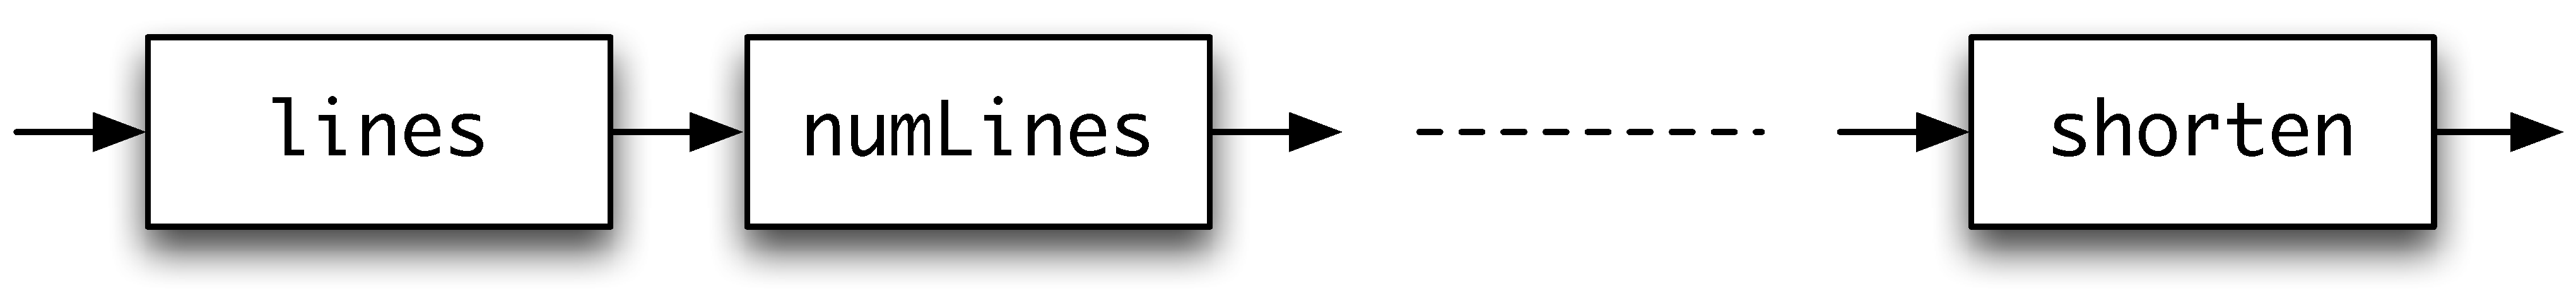
\includegraphics[width=4.5in]{Pictures/pipeline.pdf}
\end{center}
It is easy to see how designs like these can be modified. To take one example,
the indexing program above filters out short words only as its final operation.
There are a number of earlier points in the chain at which this could have been
done, and it is a worthwhile exercise to consider these.

\begin{exercises}


\item
Define the function \texttt{lines} using the functions \texttt{getUntil} and 
\texttt{dropUntil} from Chapter \ref{patternsGen}, or the built-in functions \texttt{takeWhile}
and \texttt{dropWhile}. You should be careful that your functions do not give an
empty word when there are empty lines in the \texttt{Doc}; this might happen for the
examples \texttt{"cat\bs{n}\bs{n}dog"} and \texttt{"fish\bs{n}"}.

\item
How would you use lambda expressions to replace the local definitions in
\texttt{makeLists} and \texttt{shorten}? How would you define these
functions using list comprehensions?

\item
In the index for this book, instead of printing an entry like
\begin{alltt}
cathedral        3, 5, 6, 7, 9, 10
\end{alltt}
a number of ranges could be given:
\begin{alltt}
cathedral        3, 5-7, 9-10
\end{alltt}
How would you redesign your program to do this? Hint: first think about the type
of the new index representation and then consider adding
another function to the (forward) composition which currently forms the
definition of \texttt{makeIndex}.


\item 
How would you re-define \texttt{sortLs} so that duplicate copies of an item are
{\em not\/} removed? For the index, this means that if a word occurs twice on line
\texttt{123} say, then \texttt{123} occurs twice in the index entry for that word.

\item
How could the functions \texttt{getUntil} and \texttt{dropUntil} be used in the
definition of \texttt{amalgamate}?

\item
Explain how the function \texttt{sizer} defined locally in \texttt{shorten}
can be defined as a composition of
built-in functions and operator sections; the role of \texttt{sizer} is
to pick the second half of a pair, find its length, and compare the result
with \texttt{4}.

\item
How is the following definition of the last conditional
equation for \texttt{amalgamate}
incorrect? Give an example calculation to justify your answer.
\begin{alltt}
amalgamate ((l1,w1):(l2,w2):rest)
  | w1 /= w2    = (l1,w1) : amalgamate ((l2,w2):rest)
  | otherwise   = (l1++l2,w1) : amalgamate rest
\end{alltt}

\item
Give a definition of
\begin{alltt}
printIndex :: [ ([Int],Word) ] -> IO ()
\end{alltt}
which gives a neatly laid-out printable version of an index, as shown at
the start of the section. You might find it useful to define a function 
\begin{alltt}
showIndex :: [ ([Int],Word) ] -> String
\end{alltt}
and to use this as a part of your definition of \texttt{printIndex}.

\item 
Modify the program so that words of less than four letters are removed
as a part of the
definition of \texttt{allNumWords}.

\item 
Modify the \texttt{makeIndex} function so that instead of
returning the list of line numbers on which a word occurs, the function
returns
the total number of times that the word occurs. You will need to make
sure that multiple occurrences of a word in a single line are counted. There
are two ways of tackling the problem.
\begin{titemize}
\item Modify the program as little as is necessary -- you could return the
length of a list rather than the list itself, for instance.
\item Take the program structure as a guide, and write a (simpler) program
which calculates the number of occurrences directly.
\end{titemize}

\item
Modify the program so that capitalized words like \texttt{"Dog"} are indexed under
their uncapitalized equivalents (\texttt{"dog"}). This does not work well for
proper names like \texttt{"Amelia"} --- what could you do about that?

\item
The function \texttt{sortLs} is limited to sorting lists of type 
\texttt{[(Int,Word)]} because it calls the \texttt{orderPair} function. Redefine the
function so that it takes the comparison function as a {\em parameter}. What is
its type after this redefinition?
\index{document index|)}

\item 
How would you modify the program if it was to be used to form the index
for a Haskell script? Hint: you need to think about what it is sensible to
ignore in such an enterprise.
\end{exercises}



\section{Development in practice}
\index{program development!in practice|(}

This section goes back to the advice on design and programming
from Chapter \ref{writingProgs} and illustrates how it can be used in a series of
programming examples.

\subsection*{Generalizing the problem}
\index{generalization}

Suppose that we are asked to define the lists \texttt{[1 ..\ n]} for
ourselves. A first attempt might try to use recursion, thus\minx{..}
\begin{alltt}
[1 ..\ n] = 1 : [2 ..\ n]\hfill(..1)
\end{alltt}
but the problem here is that \texttt{[2 ..\ n]} is not an instance of
what we are trying to define. The presence of the \texttt{2} here suggests 
that instead of solving the particular
problem of lists starting at \texttt{1} we should solve the more general problem
of defining lists beginning at an arbitrary value. We therefore define \texttt{[m ..\ n]}:
\begin{alltt}
[m .. n]
  | m>n         = []\hfill(..2)
  | otherwise   = m : [m+1 .. n]
\end{alltt}
Another solution is given by 
\begin{alltt}
[1 .. n] 
  | 1>n         = []\hfill(..3)
  | otherwise   = [1 .. n-1] ++ [n]
\end{alltt}
but \texttt{(..3)} has the disadvantage that it is substantially less
efficient than \texttt{(..2)}, a topic we pick up in Chapter
\ref{behaviour}.

Another example of generalization was given in the text processing
example in Section \ref{textProc} where we defined a function
\texttt{getLine}. The effect of this function is to take a list of words
and to return the list of words making up the maximal first line (of length
\texttt{lineLen}) which can be
built from the words. It was apparent in making the definition that we
needed to make the line length a parameter of the definition, so that
we defined
\begin{alltt}\minx{getLine}
getLine :: Int -> [Word] -> Line
\end{alltt}
rather than giving it the type \texttt{[Word] -> Line}.

\subsection*{Simplifying the problem}
\index{simplification}

Suppose that we are asked to solve the problem of identifying strings
which are palindromes, like
\begin{alltt}\index{palindrome}
"Madam I\bs{'}m Adam"
\end{alltt}
One way of approaching the problem is first to think of identifying
palindromes where punctuation and capitalization are not considered,
such as \texttt{"ABBA"}. We might solve this by
\begin{alltt}
simplePalCheck :: String -> Bool\label{simplePalCheck}
simplePalCheck st = (reverse st == st)
\end{alltt}
for instance, but note that there are at least two other different ways we might
implement the function \texttt{simplePalCheck}. Once we have this function we can
then {\em modify\/} it to solve the original problem. Alternatively we can {\em use\/} 
this solution to a simplified problem in the full solution:
\begin{alltt}\minx{palCheck}
palCheck = simplePalCheck . clean
\end{alltt}
where
\begin{alltt}
clean :: String -> String
\end{alltt}
puts all capitals into small letters and removes punctuation. We look at this in the next section.

\subsection*{Design choices}
\index{design!choices in}

The \texttt{clean} function combines mapping (capitals to smalls) and
filtering (removing punctuation) and so can be solved thus
\begin{alltt}
clean = map toSmall . filter notPunct\hfill(clean.1)
\end{alltt}
or by means of a list comprehension
\begin{alltt}
clean st = [ toSmall ch | ch <- st , notPunct ch ]\hfill(clean.2)
\end{alltt}
How do we choose between these options? One advantage of
\texttt{(clean.1)} is that we see clearly that we have a function
composition, but perhaps \texttt{(clean.2)} is more readable.

\subsection*{Auxiliary functions}

Suppose we are asked to define when one string is a subsequence of
another. By that we mean that the characters of the first string occur
next to each other inside the second string, so that \texttt{"Chip"} is
a subsequence of \texttt{"Fish \& Chips"}, but not of \texttt{"Chin
up"}. The function we seek to define is
\begin{alltt}\minx{subseq}
subseq :: String -> String -> Bool
\end{alltt}
and we try to define this by recursion. Starting with the cases of the
empty string,
\begin{alltt}
subseq []    _  = True
subseq (_:_) [] = False
\end{alltt}
so what is the general case, \texttt{subseq (x:xs) (y:ys)}? 
\begin{itemize}
\item One
alternative is that \texttt{(x:xs)}
is a subsequence of \texttt{ys}, as in \\
\texttt{subseq "Chip" "Fish \& Chips"}
\item The other alternative is that \texttt{(x:xs)} occurs at the start of 
\texttt{(y:ys)}, as in\\
\texttt{subseq "Chip" "Chips"}
\end{itemize}
This latter is not a recursive call to the function we are defining, so
we have to say 
\begin{alltt}
subseq (x:xs) (y:ys)
  = subseq (x:xs) ys || frontseq (x:xs) (y:ys)
\end{alltt}
and write an auxiliary function definition to check this new condition.
\begin{alltt}\minx{frontseq}
frontseq :: String -> String -> Bool
frontseq []     _  = True
frontseq (_:_)  [] = False
frontseq (x:xs) (y:ys)
  = (x==y) \&\& frontseq xs ys
\end{alltt}



\begin{exercises}


\item
Give a recursive definition of the range
\begin{alltt}
[m,n .. p]
\end{alltt}

\item
Think of two more ways of implementing the function
\begin{alltt}
simplePalCheck :: String -> Bool
\end{alltt}
discussed on page \pageref{simplePalCheck}.

\item
Define a function 
\begin{alltt}
subst :: String -> String -> String ->  String
\end{alltt}
so that the result of \texttt{subst start find replace} is the string
\texttt{start}
modified so that the first occurrence of \texttt{find} as a subsequence
is replaced by \texttt{replace}. If there is no such subsequence, the
string should be returned unmodified, so that, for instance,
\begin{alltt}
subst "Fish \& Chips" "Chip" "Boat" \step "Fish \& Boats"
subst "Fish \& Chips" "Ship" "Boat" \step "Fish \& Chips"
\end{alltt}
Modify the definition so that every occurrence of \texttt{find} is
replaced by \texttt{replace}.
Explain what your original and modified definitions do in the case of the example 
\begin{alltt}
subst "Fish \& Chips" "" "Boat"
\end{alltt}
\index{program development!in practice|)}
\end{exercises}

\section{Understanding programs}
\label{understanding}
\index{understanding programs}

This section offers advice to readers confronted with an 
unfamiliar function definition. There are various things we can do 
with the definition, and these are examined in turn here.
Given a functional program like
\begin{alltt}
mapWhile :: (a -> b) -> (a -> Bool) -> [a] -> [b]\minx{mapWhile}
\bl
mapWhile f p []    = [] \hfill (mapWhile.1)
mapWhile f p (x:xs)
  | p x            = f x : mapWhile f p xs \hfill (mapWhile.2)
  | otherwise      = [] \hfill (mapWhile.3)
\end{alltt}
we can understand what it means in various different ways. We can read
the program itself, we can write calculations of examples using
the program, we can prove properties of the program, and we can
estimate its space and time complexity,

\subsection*{Reading the program}
Besides any comments which might accompany a program, the program itself is
its most important documentation. 

The type declaration\index{type declaration}
gives information about
the input and output types: for \texttt{mapWhile}, we have to supply three
arguments:
\begin{titemize}
\item a function, \texttt{f} say, of arbitrary type, \texttt{a -> b};
\item a \textbf{property\/} of objects of type \texttt{a}; that is a function
taking an \texttt{a} to a Boolean value; and,
\item a list of items of type \texttt{a}.
\end{titemize}
The output is a list of elements of type \texttt{b} --
the output type of \texttt{f}.

The function definition itself is used to give values of \texttt{mapWhile}, but
also can be read directly as a description of the program.
\begin{titemize}
\item On \texttt{[]}, the result is \texttt{[]}.
\item On a non-empty list, if the head \texttt{x} has property \texttt{p}, then
according to \texttt{(mapWhile.2)}, we have \texttt{f x} as the first element of the
result, with the remainder given by a recursive call on \texttt{xs}.
\item If the property \texttt{p} fails of \texttt{x}, the result is terminated, as
it were, by returning the empty list \texttt{[]}.
\end{titemize}
In the definition we have a complete description of how the program behaves,
but we can animate this by trying specific examples.


\subsection*{Calculating with the program}
\index{calculation}

A more concrete view of what the program does is given by calculating
particular examples. For instance,
\begin{alltt}
mapWhile (2+) (>7) [8,12,7,13,16]
\step 2+8 : mapWhile (2+) (>7) [12,7,13,16] \hfill {\rm by} (mapWhile.2)
\step 10 : 2+12 : mapWhile (2+) (>7) [7,13,16] \hfill {\rm by} (mapWhile.2)
\step 10 : 14 : [] \hfill {\rm by} (mapWhile.3)
\step [10,14]
\end{alltt}
Other examples include
\begin{alltt}
mapWhile (2+) (>2) [8,12,7,13,16] \step [10,14,9,15,18]
mapWhile (2+) (>2) []             \step []
\end{alltt}
Note that in these examples we use \texttt{mapWhile} at the instance
\begin{alltt}
(Int -> Int) -> (Int -> Bool) -> [Int] -> [Int]
\end{alltt} 
of its polymorphic type,
given by replacing the type variables \texttt{a} and \texttt{b} by the type 
\texttt{Int}.

\subsection*{Reasoning about the program}
\index{proof}

We can get a deeper understanding about a program by \textbf{proving} properties
that the program might have. For \texttt{mapWhile}, we might prove that for all
\texttt{f}, \texttt{p} and finite lists \texttt{xs},
\begin{alltt}
mapWhile f p xs            = map f (takeWhile p xs)\hfill(mapWhile.4)
mapWhile f (const True) xs = map f xs\hfill(mapWhile.5)
mapWhile id p xs           = takeWhile p xs\hfill(mapWhile.6)
\end{alltt}
where we can, in fact, see \texttt{(mapWhile.5)} and \texttt{(mapWhile.6)} as consequences of the
characterization of \texttt{mapWhile} given by property \texttt{(mapWhile.4)}. 

Rather than proving these properties, it is possible to use QuickCheck to test them with random data. Recall the discussion in the breakout box `QuickCheck and higher-order functions'  on page \pageref{QChofs},\index{QuickCheck} which outlines how functions of this sort can be tested on a selection of functional arguments and randomly-generated list data.


\subsection*{Program behaviour}
\index{behaviour}
It is not hard to see that the program will at worst take time linear (that is
\texttt{O(n\uppp{1})}) in the length (\texttt{n}) of the list argument assuming \texttt{O(n\uppp{0})}
behaviour of \texttt{f} and \texttt{p}, as it runs through the elements of the list
once, if at all.

The \textbf{space\/} behaviour is more interesting; because we can output the
head of a list once produced, the space required will be constant, as
suggested by underlining the parts which can be output in the calculation
above.
\begin{alltt}
mapWhile (2+) (>7) [8,12,7,13,16]
\step 2+8 : mapWhile (2+) (>7) [12,7,13,16] 
\step \underline{10} : 2+12 : mapWhile (2+) (>7) [7,13,16] 
\step \underline{10 : 14} : [] 
\step \underline{[10,14]}
\end{alltt}
We return to a fuller discussion of program behaviour in Chapter \ref{behaviour}.

\subsection*{Getting started}

Each view of the program gives us a different understanding of its
behaviour, but when we are presented with an unfamiliar definition we can
begin to understand what its effect is by calculating various small examples.
If we are given a collection of functions, we can test out the functions from
the bottom up, building one calculation on top of another, using GHCi as a calculator. 
 
The important
thing is to realize that rather than being stuck, we can get started by
calculating representative examples to show us the way.

\begin{summary}
This chapter has explored the idea that program development works in a cycle: first we
clarify the specification of the problem to be solved, next we devise a
plan of how to solve the problem, and only then do we implement the
solution. 

At each stage we should reflect on and evaluate what we have
done: this aspect is crucial particularly when we are learning to
program. For example, being aware of the errors that we make can help us to prevent
making them in the future. Also, if we take a problem we have already solved and 
try to solve it with a new technique we will learn something about the new technique
as well as seeing how it fits in with what we have learned already. This is
something that we do by continually revisiting the \texttt{Picture}
case study.

\index{program development|)}
\end{summary}

%\end{document}
